
	\begin{questions}
		
	
		\question[2] Sur une courbe qui représente l'évolution de la température en fonction du temps, comment s'appelle la partie horizontale ?
		
		\fillwithdottedlines{1.5cm}  
		
	
		
		\question[2] Quelle propriété d'un corps change lorsqu'il change d'état ?
		
		\fillwithdottedlines{1.5cm}  
		
		\question[6] La courbe suivante décrit l'évolution de la température d'un corps lors d'un changement d'état :
		
		\begin{center}
			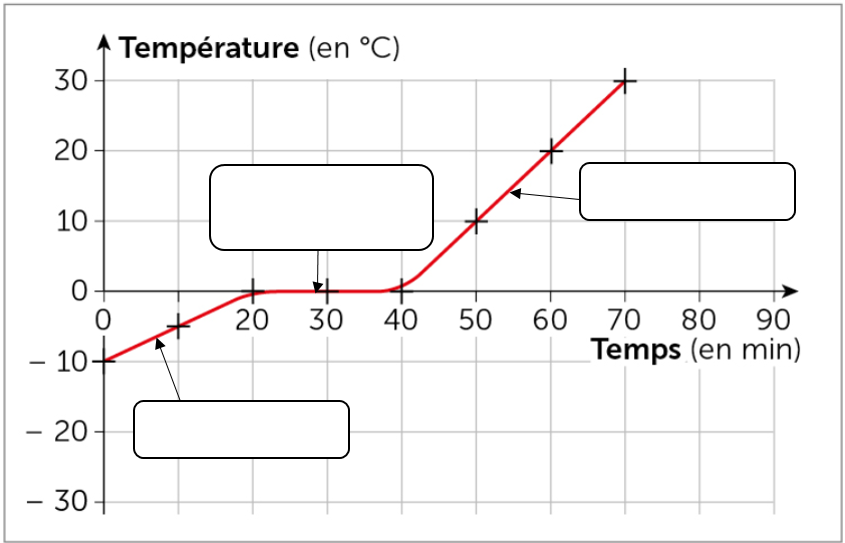
\includegraphics[scale=0.65]{courbe}
		\end{center}
	
		\begin{parts}
			\part[4] Préciser dans chacun des états indiqués l'état dans lequel se trouve le corps.
			
			\part[2] Quel changement d'état à lieu ici ;
			\fillwithdottedlines{1cm} 
		\end{parts}
	
	
		\question[2] Comment s'appelle le passage de l'état solide à liquide ?
		\fillwithdottedlines{1.5cm}
		
		\question[2] Pendant un changement d'état, la température d'un corps :
		\begin{checkboxes}
			\choice diminue
			\correctchoice ne change pas
			\choice augmente
		\end{checkboxes}
	
		\vspace*{1cm}
		\question[2] Lorsque l'on fournit de l'énergie à de l'eau à 25 °C :
		\begin{checkboxes}
			\choice elle change d'état
			\choice sa température reste constante
			\correctchoice sa température augmente
		\end{checkboxes}
	
		\vspace*{1cm}
		\question[2] Dans des conditions normales de température et de pression, quelle est la température de fusion de l'eau ?
		
		\fillwithdottedlines{1.5cm}
		
		
			\question[2] L'évaporation et l'ébullition correspondent au même changement d'état, lequel ?
		
		\fillwithdottedlines{1.5cm}  
	\end{questions}
	
